\documentclass{article}

\usepackage{cmlgc}
\usepackage{enumitem}
\usepackage{graphicx}
\usepackage{geometry}
\geometry{
    a4paper
}
\usepackage{hyperref}
\hypersetup{
    colorlinks=true,
    linkcolor=blue,
    urlcolor=blue
}
 
\begin{document}
\newgeometry{
    top=8mm,
    bottom=8mm,
    left=3mm,
    right=8mm
}
\begin{minipage}{0.8\textwidth}
\begin{flushleft}
    \begin{minipage}{1\textwidth}
        \begin{minipage}{.5\textwidth}
            \vspace{.2cm}
            {\huge \textbf{Vadim \textsc{Bertrand}}}\\[.3 cm]
            \url{https://github.com/vadmbertr/}
        \end{minipage}
        \begin{minipage}{.5\textwidth}
        \begin{flushright}
            \begin{minipage}{.74\textwidth}
            \begin{flushright}
                \href{tel:33614623218}{+33 6 14 62 32 18} \\[.1 cm]
                \href{mailto:vadim.bertrand@gmail.com}{vadim.bertrand@gmail.com} \\[.1 cm]
                Grenoble area \\[.1 cm]
                FRANCE
            \end{flushright}
            \end{minipage}
            \begin{minipage}{.24\textwidth}
            \begin{flushright}
                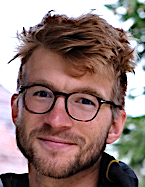
\includegraphics[width=1\textwidth]{picture.png}
            \end{flushright}
            \end{minipage}
        \end{flushright}
        \end{minipage}
    \end{minipage}
    \\[.3 cm]
    \textbf{Statistics and Data Sciences 2\textsuperscript{nd} year Master Student – Software Engineer}
    \\[.5 cm]
    \section*{\textsc{Education}}
    \begin{itemize}
        \item \textbf{2022 – 2023\qquad \qquad \qquad \qquad Université Grenoble Alpes – IM\textsuperscript{2}AG} \\
        2\textsuperscript{nd} year Master’s in Statistics and Data Sciences – Labelled “Core IA” by MIAI
        \vspace{-.15cm}
        \begin{itemize}[leftmargin=*]
        \setlength\itemsep{.01cm}
            \item Bayesian statistics
            \item Computational statistics: bootstrap, Monte Carlo, permutation
            \item Non-parametric and functional estimation
            \item Operations research and optimization
            \item Spatial statistics (stochastic processes)
            \item Supervised learning: Neural Networks, random forest, Support Vector Machine
        \end{itemize}
        \item \textbf{2021 – 2022\qquad \qquad \qquad \qquad Université Grenoble Alpes – IM\textsuperscript{2}AG} \\
        1\textsuperscript{st} year Master’s in Statistics and Data Sciences – Labelled “Core IA” by MIAI
        \vspace{-.15cm}
        \begin{itemize}[leftmargin=*]
        \setlength\itemsep{.01cm}
            \item Probability, inferential statistics and statistical tests
            \item Time series analysis
            \item Unsupervised \textit{- hierarchical clustering, k-means -} and supervised \textit{- (G)LM, kNN, LDA/QDA, Lasso/Ridge/Elastic-Net -} learning
        \end{itemize}
        \item \textbf{2011 – 2014\qquad \qquad \qquad \qquad Grenoble INP – Phelma / Ensimag} \\
        Engineering degree “Internet, Services and Connected Systems”
    \end{itemize}
    \section*{\textsc{Academic and Professional Experience}}
    \begin{itemize}
        \item \textbf{March 2023 – Aug. 2023 \quad Research Internship – MAGe team of TIMC – Grenoble} \\
        “Exploration of joint deconvolution algorithms for omic data” – 2\textsuperscript{nd} year Master’s – \textbf{\textit{ \href{https://vadmbertr.github.io/Exploration-of-joint-deconvolution-algorithms-for-omic-data/M2_Internship_report__Exploration_of_joint_deconvolution_algorithms_for_omic_data.pdf}{report}}}
        \vspace{-.15cm}
        \begin{itemize}[leftmargin=*]
        \setlength\itemsep{.01cm}
            \item Constructed and ran a comprehensive benchmark to evaluate deconvolution pipelines
            \item Introduced and evaluated two novel multi-omics integration strategies
            \item Presented a \href{https://vadmbertr.github.io/Exploration-of-joint-deconvolution-algorithms-for-omic-data/poster_jobim_ismb.pdf}{poster} at JOBIM and ISMB conferences
        \end{itemize}
        \item \textbf{Nov. 2022 – Feb. 2023 \qquad Tutored project – 2\textsuperscript{nd} year Master’s}
        \vspace{-.15cm}
        \begin{itemize}[leftmargin=*]
        \setlength\itemsep{.01cm}
            \item Effect of human disturbance on narwhals feeding
            \vspace{-.15cm}
            \begin{itemize}[leftmargin=*]
            \setlength\itemsep{.01cm}
                \item Used of Poisson process, GLM and mixed-models for modelling
                \item Constructed confidence intervals through a Monte Carlo procedure
            \end{itemize}
            \item Estimating the age of narwhals from their tusk grooves
            \vspace{-.15cm}
            \begin{itemize}[leftmargin=*]
            \setlength\itemsep{.01cm}
                \item Modelling by a double sine composed with a Ornstein-Uhlenbeck process
                \item Identifiability simulation using SAEM algorithm with a MCMC step
            \end{itemize}
        \end{itemize}
        \item \textbf{May 2022 – Aug. 2022 \qquad Research Internship – DAO team of LJK – Grenoble} \\
        “Deep generative learning for next-generation drugs” – 1\textsuperscript{st} year Master’s – \textbf{\textit{ \href{https://vadmbertr.github.io/Deep-generative-learning-for-next-generation-drugs/Internship_report___Deep_generative_learning_for_next_generation_drugs.pdf}{report}}}
        \vspace{-.15cm}
        \begin{itemize}[leftmargin=*]
        \setlength\itemsep{.01cm}
            \item Extended a 2D image inpainting CNN to 3D and drugs generation tasks
            \item Used an invariant ligand-protein complex representation based on oriented residue density grids
            \item Implemented using PyTorch library
        \end{itemize}
        \item \textbf{Sept. 2016 – Aug. 2021 \qquad Engineer – DANCE team (CNRS / Inria) – Grenoble}
        \vspace{-.15cm}
        \begin{itemize}[leftmargin=*]
        \setlength\itemsep{.01cm}
            \item Developed, deployed and maintained applications for collecting, estimating and predicting road traffic indicators in real time in the Grenoble Metropolis via the use of models designed by members of the team
            \vspace{-.15cm}
            \begin{itemize}[leftmargin=*]
            \setlength\itemsep{.01cm}
                \item \url{http://gtl.inrialpes.fr} (stable)
                \item \url{http://gtlville.inrialpes.fr} (experimental)
            \end{itemize}
            \item Collaborated with PhD / post-doctoral students and supervised interns
                \vspace{-.15cm}
                \begin{itemize}[leftmargin=*]
                \setlength\itemsep{.01cm}
                    \item Built a dynamic partition model – based on nodes’ state – of a road network to estimate travel times through the obtained partitions – \textbf{\textit{\href{https://hal.archives-ouvertes.fr/hal-01953560}{paper}}}
                \end{itemize}
            \item Wrote technical documentation for the opening of a public tender to collect traffic data
        \end{itemize}
    \end{itemize}
\end{flushleft}
\end{minipage}
\hfill\vline\hfill
\begin{minipage}{0.15\textwidth}
    \begin{minipage}{1\textwidth}
    \begin{flushleft}
        \textbf{1994} \\
        First snowplows \\[.2cm]
        \textbf{1996} \\
        Judo white belt \\[.2cm]
        \textbf{1998} \\
        Initiation to rugby \\[.9cm]
        \textbf{2007} \\
        Sport-study rugby program \\[.5cm]
        \textbf{2012} \\
        3 months in Australia \\[.2cm]
        \textbf{2014} \\
        Switch to ski touring \\[.1cm]
        \textbf{2015} \\
        2 months around the Balkans \\[.2cm]
        \textbf{2017} \\
        Transition to Touch rugby \\[.2cm]
        \textbf{2019} \\
        Rediscover chess \\[.1cm]
        \textbf{2020} \\
        1\textsuperscript{st} diving level \\[.1cm]
        \textbf{2021} \\
        Join the french M30 touch rugby selection \\[.2cm]
        \textbf{2023} \\
        Silver medal at the European Touch Championships
    \end{flushleft}
    \end{minipage}
    \begin{minipage}{1\textwidth}
    \vspace{7.1cm}
    \begin{flushleft}
        \textbf{Languages} \\[.1cm]
        English \quad Fluent \\
        Spanish \quad Notions
    \end{flushleft}
    \end{minipage}
    \begin{minipage}{1\textwidth}
    \vspace{1cm}
    \begin{flushleft}
        \textbf{Miscellaneous} \\[.1cm]
        Python, R, Julia \\
        \LaTeX \\
        Git \\
        Shell scripting
    \end{flushleft}
    \end{minipage}
\end{minipage}

\end{document}
